\begin{figure}[H]
    \centering
    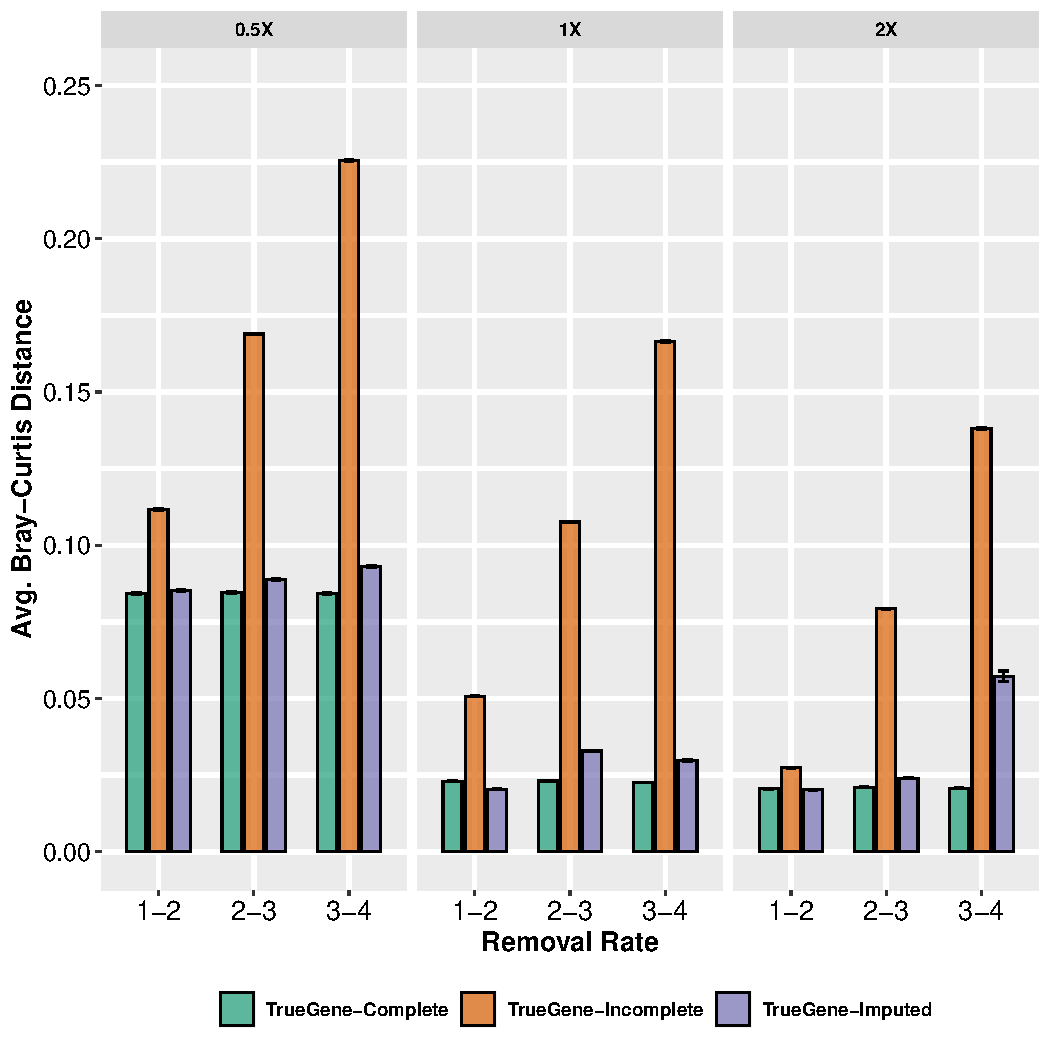
\includegraphics[width=\linewidth]{37_Taxon_Dataset/plot_BRC.pdf}
    \caption{The Bray-Curtis Distance between the quartet distributions of true gene trees and the complete, incomplete and the imputed gene trees for three taxa removal rate  i.e. 1-2, 2-3 and 3-4 taxa respectively.}
    \label{fig:BRC_37_taxon}
\end{figure}

\begin{figure}[H]
    \centering
    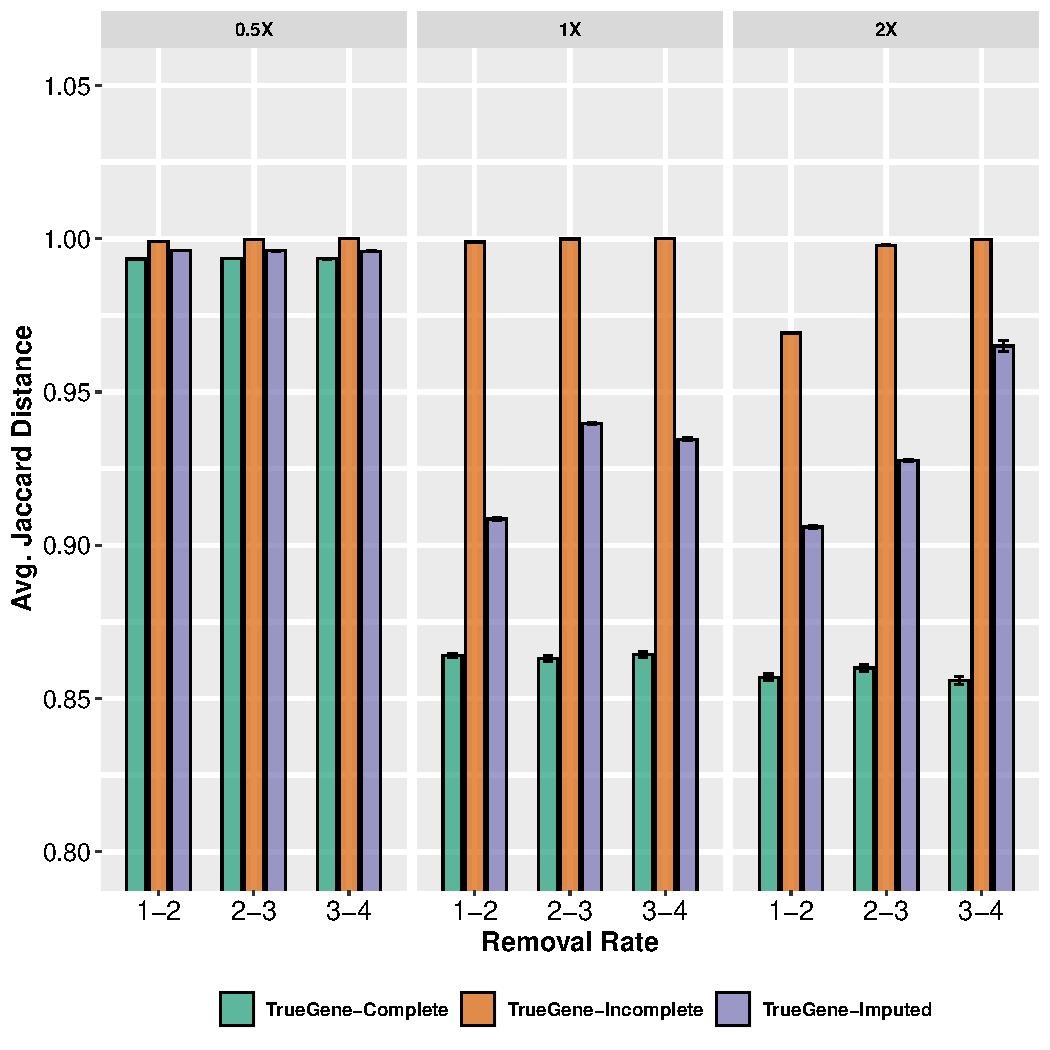
\includegraphics[width=\linewidth]{37_Taxon_Dataset/plot_JAC.pdf}
    \caption{The Jaccard Distance between the quartet distributions of true gene trees and the complete, incomplete and the imputed gene trees for three taxa removal rate  i.e. 1-2, 2-3 and 3-4 taxa respectively.}
    \label{fig:JAC_37_taxon}
\end{figure}

\begin{figure}[H]
    
    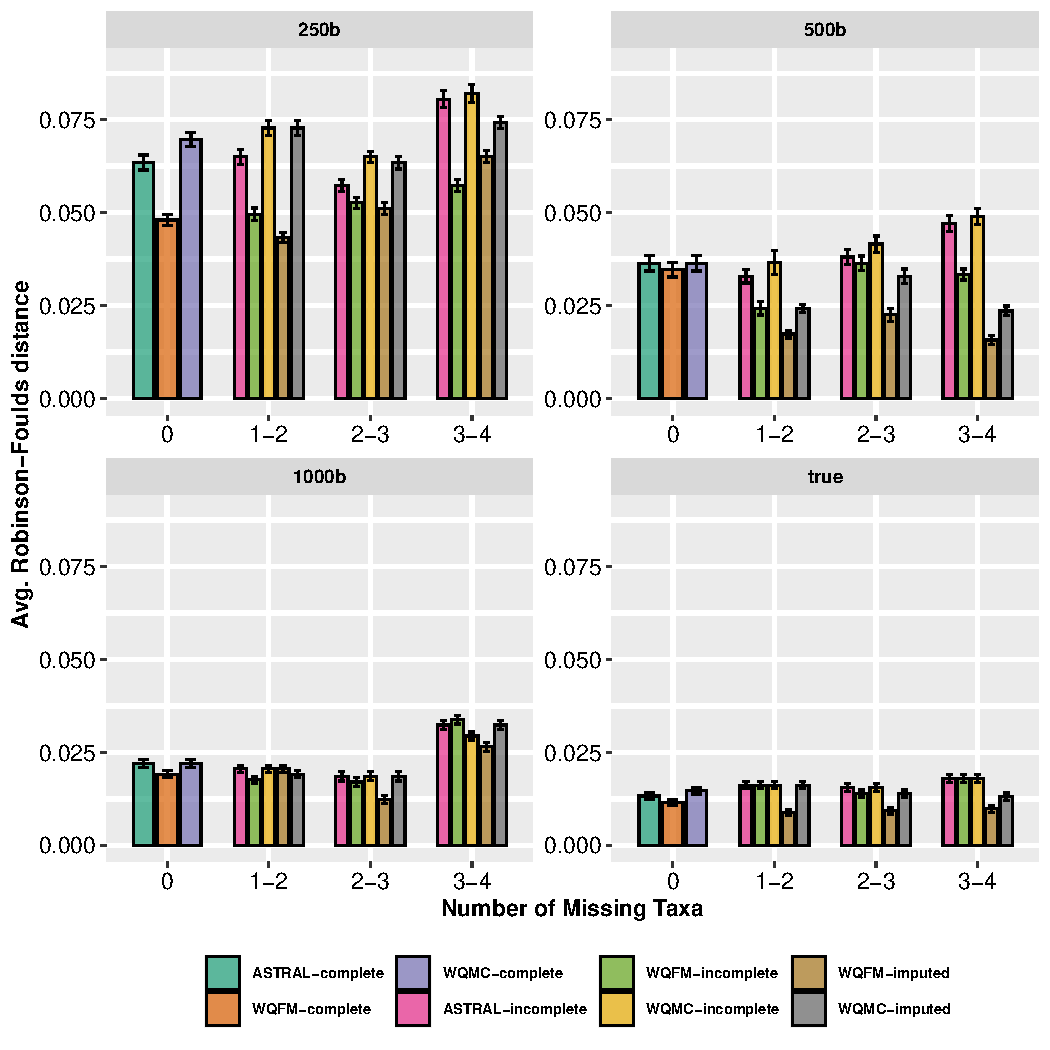
\includegraphics[width=\linewidth]{37_Taxon_Dataset/SequenceLength/plot_QRF_All.pdf}
    \caption{Average Robinson-Foulds distance of Complete(ASTRAL), Complete(WQMC), 
    Incomplete(Astral), Incomplete(WQMC) and Imputed(WQMC) on the \textbf{37-taxon} dataset with different taxa removal rate. We varied the taxa removal from ($6-13\%$) to ($33-40\%$). We analyzed the estimated gene trees only. We show the average RF distance with standard error bars over 20 replicates.}
    \label{fig:RF_Rates_37_Taxon_seqLength_All}
\end{figure}
